% PROGETTAZIONE E CODIFICA

\chapter{Progettazione e codifica}\label{chap:design}

\section {Progettazione architetturale}

\section{Progettazione grafica}
Prima di procedere alla definizione delle classi necessarie per l'implementazione 
dell'applicazione è stato deciso di effettuare la progettazione grafica della UI per far 
si che il progetto di stage abbracciasse a 360 gradi il processo di sviluppo di 
un'applicazione da parte di un'azienda.

\subsection{Wireframe}
In base ai requisiti e agli use case raccolti è stato definito il modello iniziale
 dell'applicazione tramite la realizzazione dei wireframe delle varie schermate. \\
Questo studio è la prima rappresentazione visuale dell'applicazione ed ha lo 
scopo di identificare la struttura, l'architettura dell'informazione e la 
disposizione degli elementi nella pagina.\\
Di seguito vengono riportati i wireframe sviluppati di alcune delle pagine più 
importanti di Teamwork:
\begin{figure}[H] 
	\centering
	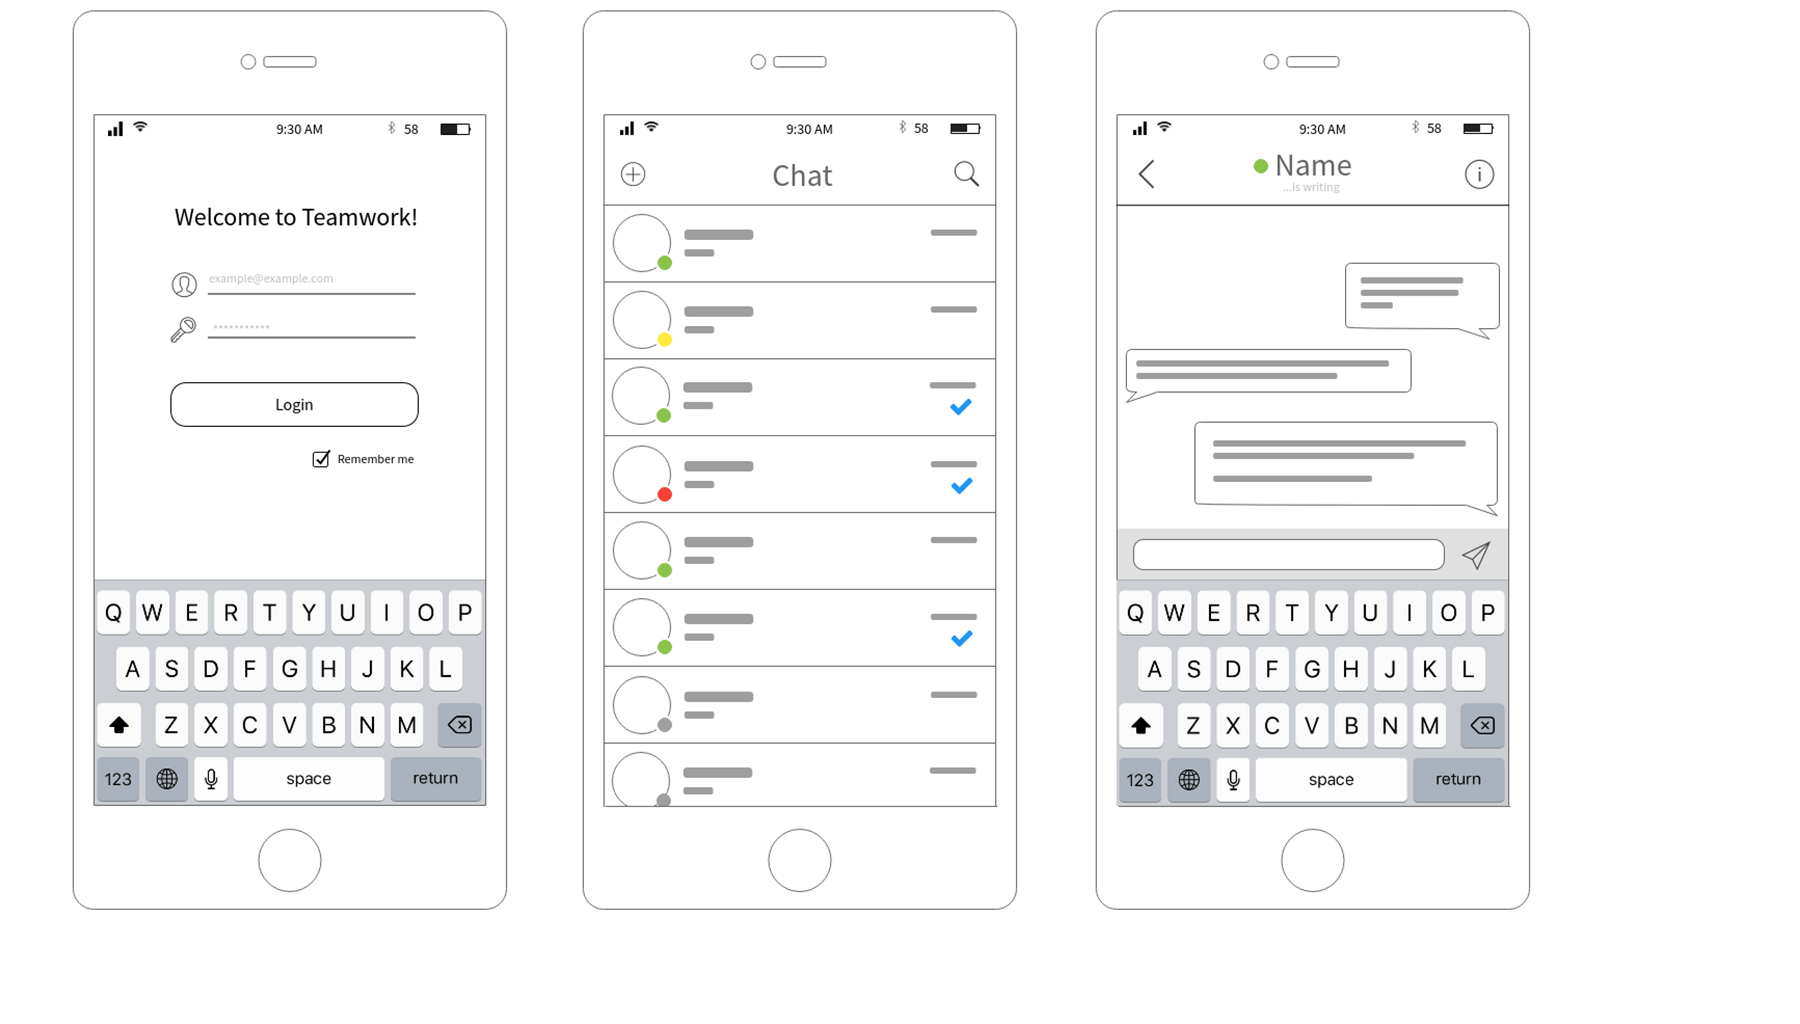
\includegraphics[scale=0.5]{wireframe}
	\caption{Wireframe pagina di login, buddylist e chat page.}
\end{figure}
Come possiamo notare dagli esempi riportati, in questa fase non è stato deciso 
nulla riguardo la rappresentazione grafica dei vari elementi. 
Si è definita soltanto la struttura delle varie schermate, il collegamento tra 
di esse e quali elementi realmente soddisfino i requisiti già studiati. 
Il risultato, comunque, è stato molto vicino alla GUI ottenuta alla fine della 
codifica in quando i wireframe sono stati disegnati tenendo conto della 
soluzione web già presente.\\ 
Questo passo è stato essenziale per farsi un'idea più chiara di come proseguire 
per ottenere il risultato desiderato.

\subsection{Linee guida}
Per quanto riguarda la GUI vera e propria sono state fornite dall'azienda delle 
guidelines da seguire per la rappresentazione grafica di ogni elemento. \\
Nello specifico le guidelines toccano temi come:
\begin{itemize}
	\item le proporzioni tra i componenti;
	\item i colori da utilizzare;
	\item le definizioni di alcuni elementi base;
\end{itemize}
Questo serve per avere uno stile comune tra le varie applicazioni che 
l'azienda sviluppa. \\
Un esempio è la definizione del componente "card", destinato alla 
visualizzazione dei dettagli relativi ad un buddy:
\begin{figure}[H] 
	\centering
	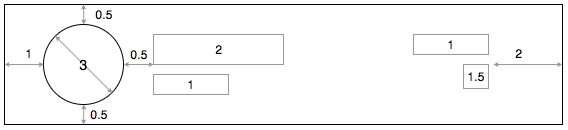
\includegraphics[scale=0.5]{guidelines}
	\caption{Esempio guidelines spazi}
\end{figure}
Si noti come ogni elemento sia posizionato in modo preciso definendo delle 
proporzioni tra gli spazi. In questo modo la successiva codifica dello stile sarà 
assolutamente definita da regole precise in modo da non dover interagire in modo 
continuativo con il responsabile grafico del progetto. \\
L'applicazione delle guidelines nel codice è avvenuta in parallelo con lo sviluppo 
in quando, seguendo una metodologia agile, si è ritenuto opportuno che le varie 
versioni prototipali dell'applicazione avessero anche una progressiva applicazione 
delle regole di stile.

\section{Progettazione di dettaglio}
Approvati questi wireframe è stato potuto proseguire alla definizione di tutti 
e soli i componenti veramente utili al layout deciso.